\section{Regime detection: real data and known change dates}
\label{sec:regime}\label{app:regime}

\paragraph{What the real data can show.} The plan predicted two things
about the detector (claim D1). Without it, CRPS would be about
\R{c/d1-detector-pred}\% better at \hC\ days when nothing changes, and
coverage would be much worse in the four weeks after a change. Berka has
no record of when a person's spending actually changed. Both strata are
therefore defined by the \emph{full model's own} alarms: origins are
selected because the detector fired or stayed silent, and the
detector-off forecast is then judged on origins chosen by the detector-on
model. A false alarm, whose jump widens the cone for nothing, lands in the
``after a change'' stratum by construction. The comparison in these
strata is therefore descriptive only.

Descriptively, at origins with no alarm in the previous four weeks,
removing the detector raises CRPS: skill
\R{ho/ablp/no-recent-alarm/abl-no-detector/90/skill@3}
[\R{ho/ablp/no-recent-alarm/abl-no-detector/90/skill_lo@3},
\R{ho/ablp/no-recent-alarm/abl-no-detector/90/skill_hi@3}] at \hC\ days
(positive would mean the detector-free model is better). At origins within
four weeks after an alarm, removing it raises \lC\% coverage, by
\R{ho/ablp/regime-alarm-in-last-28-days/abl-no-detector/30/cov90_diff} and
\R{ho/ablp/regime-alarm-in-last-28-days/abl-no-detector/90/cov90_diff}
points at \hB\ and \hC\ days. Over all origins, which no alarm selects,
removing the detector raises CRPS slightly
(\R{ho/ablp/all/abl-no-detector/30/skill@3} and
\R{ho/ablp/all/abl-no-detector/90/skill@3}). These numbers cannot
separate ``the detector reacts to noise'' from ``Berka has few sustained
changes of the kind the detector models''.

\paragraph{The clean test: known change dates.} The synthetic sweep steps
the spending rate or the paycheck by a known factor on a known day, and
forecasts from origins before and after it, with the detector on and off,
over \R{c/regime-seeds} seeds per scenario (Table~\ref{tab:detection},
Figure~\ref{fig:detector}).
\begin{itemize}
\item \textbf{Large changes on model-matched data: a large benefit.} After
  spending doubles, the \hB-day \lC\% interval covers
  \R{syn/cov/matched-spend-x2/14/detector/30/cov90}\% from
  \R{c/settle-days} days after the change with the detector, against
  \R{syn/cov/matched-spend-x2/14/no-detector/30/cov90}\% without it. CRPS
  improves by \R{syn/rpair/matched-spend-x2/14/30/skill}
  [\R{syn/rpair/matched-spend-x2/14/30/skill_lo},
  \R{syn/rpair/matched-spend-x2/14/30/skill_hi}] in skill.
\item \textbf{The first week stays overconfident.} Seven days after a
  doubling, coverage is \R{syn/cov/matched-spend-x2/7/detector/30/cov90}\%
  (model-matched) and \R{syn/cov/realistic-spend-x2/7/detector/30/cov90}\%
  (realistic). Detection needs the CUSUM's delay, a median of
  \R{syn/det/matched-spend-x2/detector/median_detect_days} and
  \R{syn/det/realistic-spend-x2/detector/median_detect_days} days.
\item \textbf{Realistic data: coverage; the CRPS effect is imprecise.}
  After a doubling on the realistic generator the detector restores much
  of the coverage (\R{syn/cov/realistic-spend-x2/28/detector/30/cov90}\%
  against \R{syn/cov/realistic-spend-x2/28/no-detector/30/cov90}\% four
  weeks after). Its effect on CRPS is imprecisely estimated:
  \R{syn/rpair/realistic-spend-x2/28/30/skill}
  [\R{syn/rpair/realistic-spend-x2/28/30/skill_lo},
  \R{syn/rpair/realistic-spend-x2/28/30/skill_hi}].
\item \textbf{Halved spending on realistic data is effectively never
  detected} (\R{syn/det/realistic-spend-x0.5/detector/detected_share}\% of
  runs). Here the detector \emph{costs} CRPS around the change. The
  skill is \R{syn/rpair/realistic-spend-x0.5/m14/30/skill}
  [\R{syn/rpair/realistic-spend-x0.5/m14/30/skill_lo},
  \R{syn/rpair/realistic-spend-x0.5/m14/30/skill_hi}] from two weeks
  before, a forecast window that spans the change; its false alarms widen
  the cone without catching the change.
\item \textbf{Before a change, on model-matched data, there is no
  measurable cost.} Skill is \R{syn/rpair/matched-spend-x2/m28/30/skill}
  four weeks before a doubling. The false-alarm rate in runs with no step
  is \R{d/fa-matched} a year on model-matched data and \R{d/fa-realistic}
  on realistic data.
\end{itemize}
So, on synthetic data with known change dates, the detector helps after
large changes when the data resemble the model, and it is weak for
downward changes in skewed spending. Whether it helps after true changes
on real accounts, these data cannot say.
\begin{figure}[t]
\centering
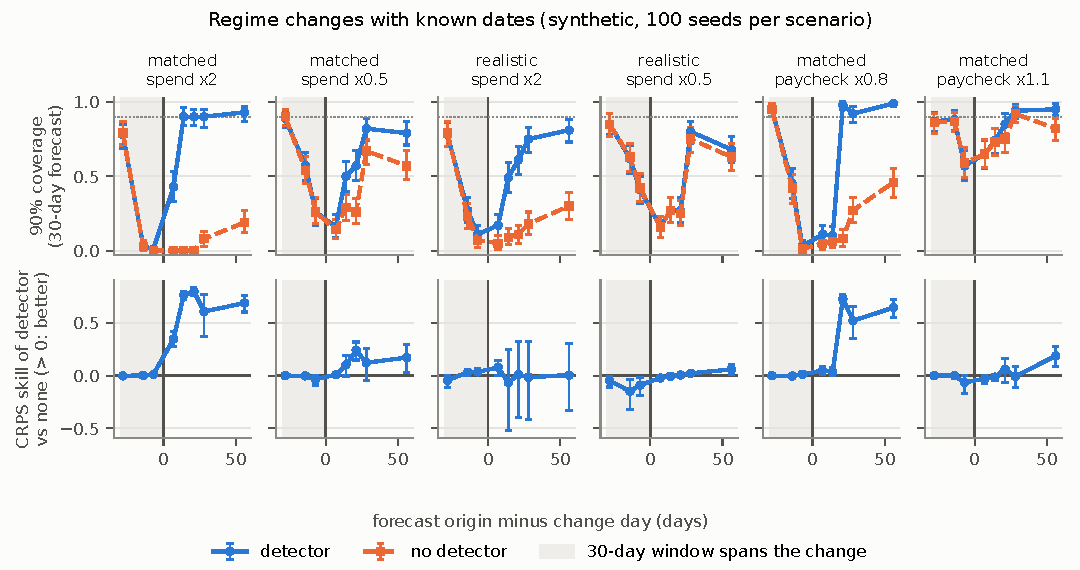
\includegraphics[width=\linewidth]{figures/detector-synthetic.pdf}
\caption{Detector on and off around a known change (synthetic, \hB-day
forecasts, \R{c/ci-level}\% seed-bootstrap intervals). Top: \lC\% coverage.
Bottom: paired CRPS skill of the detector (positive: detector better).
Shaded origins forecast across the change, which no method here can
anticipate.}
\label{fig:detector}
\end{figure}

\subsection{The planned ablations of V0 (claim D1)}
\label{sec:ablations}

Each ablation removes one component, and its forecasts are compared with
the full model on the same origins. The run covers all
\R{ho/abldata/accounts_with_eligible_origin} held-out accounts with eligible
origins (Table~\ref{tab:ablations}). Two caveats come first.
\begin{enumerate}[label=(\roman*)]
\item \textbf{The components were removed from V0, not from V2.} D1 was
  written into the plan before V2 existed. The ablations therefore show what
  each component does inside the original model. They do not show what it
  does inside V2, whose spending model replaces the smooth rate and the
  lumps.
\item \textbf{The alarm-defined strata are circular} (\S\ref{sec:regime}).
  They are selected by the full model's own detector.
\end{enumerate}
They were also run after the main held-out results were known, in a
second logged run, because the first run omitted them
(\S\ref{sec:timeline}).

\begin{table}[t]
\centering\scriptsize\setlength{\tabcolsep}{3.5pt}
\tab{heldout-ablations}
\caption{Held-out ablations against V0, from the separately logged ablation
run, over the origins both made: \R{ho/abldata/eligible_origins} origins in
\R{ho/abldata/accounts_with_eligible_origin} accounts per horizon (all
origins). The alarm strata are subsets of these. Skill: the ablation's
CRPS skill against V0, as the mean of per-account ratios (positive: the
ablation is better). $\Delta$cov90: the
ablation's \lC\% coverage minus V0's, in points. Columns are horizons
(days). Intervals are in the result files.}
\label{tab:ablations}
\end{table}

\begin{itemize}
\item \textbf{Adaptive noise off (fixed priors).} The prediction was worse
  coverage. Coverage does fall at \hA\ and \hC\ days
  (\R{ho/ablp/all/abl-fixed-noise/7/cov90_diff} and
  \R{ho/ablp/all/abl-fixed-noise/90/cov90_diff} points) and is unchanged
  at \hB, so the prediction holds. But CRPS is \emph{better} without
  adaptation: skill \R{ho/ablp/all/abl-fixed-noise/30/skill@3} and
  \R{ho/ablp/all/abl-fixed-noise/90/skill@3} at \hB\ and \hC\ days.
\item \textbf{Lumps off.} The prediction was under-coverage at the wide
  levels, mostly at long horizons. It holds strongly: \lC\% coverage falls
  by \R{ho/ablp/all/abl-no-lumps/30/cov90_diff} and
  \R{ho/ablp/all/abl-no-lumps/90/cov90_diff} points at \hB\ and \hC\ days.
  On sparse Berka spending, the lump resampling carries much of V0's
  spread.
\item \textbf{Spend floor off.} The prediction was no change except where
  the floor binds. It holds overall: effects stay below one point of
  coverage and below one percent of CRPS. After alarms, CRPS is worse
  without the floor
  (\R{ho/ablp/regime-alarm-in-last-28-days/abl-no-floor/90/skill@3} at
  \hC\ days), which fits the floor binding where the estimated rate has
  just jumped.
\item \textbf{Detector off.} Both predicted signs are reversed
  (\S\ref{sec:regime}). By the plan's rule as written, this falsifies
  the detector's claim. Because both strata are selected by the detector's
  own alarms, we read the result as descriptive, not as evidence about
  true changes.
\item \textbf{Noise-variance draws off.} No prediction was registered.
  The effects are negligible:
  \R{ho/ablp/all/abl-no-var-draw/90/skill@3} in skill and
  \R{ho/ablp/all/abl-no-var-draw/90/cov90_diff} points of coverage at
  \hC\ days.
\end{itemize}

\begin{table}[h]
\centering\footnotesize
\tab{synthetic-detection}
\caption{Regime detection on synthetic data with a known change day
(\R{c/regime-seeds} seeds per scenario, detector on). Recovery: the estimate
stays within a quarter of the step for \R{c/settle-days} days. False alarms
are counted in the same seeds with no step.}
\label{tab:detection}
\end{table}
